%% Based on a TeXnicCenter-Template by Tino Weinkauf.
%%%%%%%%%%%%%%%%%%%%%%%%%%%%%%%%%%%%%%%%%%%%%%%%%%%%%%%%%%%%%

%%%%%%%%%%%%%%%%%%%%%%%%%%%%%%%%%%%%%%%%%%%%%%%%%%%%%%%%%%%%%
%% HEADER
%%%%%%%%%%%%%%%%%%%%%%%%%%%%%%%%%%%%%%%%%%%%%%%%%%%%%%%%%%%%%
\documentclass[a4paper,twoside,11pt]{article}
% Alternative Options:
%	Paper Size: a4paper / a5paper / b5paper / letterpaper / legalpaper / executivepaper
% Duplex: oneside / twoside
% Base Font Size: 10pt / 11pt / 12pt


%% Language %%%%%%%%%%%%%%%%%%%%%%%%%%%%%%%%%%%%%%%%%%%%%%%%%
%%\usepackage[USenglish]{babel} %francais, polish, spanish, ...
\usepackage[T1]{fontenc}
%%\usepackage[ansinew]{inputenc}
%%\usepackage[utf8x]{inputenc}
%%\usepackage{polyglossia}
%%\setdefaultlanguage[babelshorthands]{USenglish}

\usepackage{lmodern} %Type1-font for non-english texts and characters

%% NG: Try the following for sans serif.
%% Well - take your pick. helvet leaves math in serif. But is otherwise rather nice?
%%\usepackage[scaled]{helvet}
%%\usepackage[math]{kurier}  %% Not nice.
%%\usepackage[math]{iwona}   %% Not nice.
%%\usepackage{cmbright}      %% Still will not work after installing hfbright.
%%\renewcommand*\familydefault{\sfdefault}

\usepackage{eulervm}
\usepackage{url}

%% NG: Try this for colour.
\usepackage{color}

\usepackage{float}

%% NG: Try this for HTML output
%% Also choose LaTeX => HTML of course ...
%%\usepackage[html]{tex4ht}

%% Packages for Graphics & Figures %%%%%%%%%%%%%%%%%%%%%%%%%%
\usepackage{graphicx} %%For loading graphic files
%\usepackage{subfig} %%Subfigures inside a figure
%\usepackage{tikz} %%Generate vector graphics from within LaTeX

%% Please note:
%% Images can be included using \includegraphics{filename}
%% resp. using the dialog in the Insert menu.
%% 
%% The mode "LaTeX => PDF" allows the following formats:
%%   .jpg  .png  .pdf  .mps
%% 
%% The modes "LaTeX => DVI", "LaTeX => PS" und "LaTeX => PS => PDF"
%% allow the following formats:
%%   .eps  .ps  .bmp  .pict  .pntg

%% NG: Try this to scale graphics to be at most the line length wide.
%% \includegraphics[width=\maxwidth]{figure}
\makeatletter
\def\maxwidth{%
  \ifdim\Gin@nat@width>\linewidth
    \linewidth
  \else
    \Gin@nat@width
  \fi
}
\makeatother

%% NG: Try fancy chapter headings.
%% This is Ulf Lindgren's FncyChap package. But set to Sans.
%\usepackage[Lenny]{fncychap}
%\ChTitleVar{\Huge\bfseries\sf}
%\usepackage[Glenn]{fncychap}
%\ChTitleVar{\Large\bfseries\sf}

%% NG: And we might want text in a box.
\usepackage{boxedminipage}

%% Math Packages %%%%%%%%%%%%%%%%%%%%%%%%%%%%%%%%%%%%%%%%%%%%
\usepackage{amsmath}
%%\usepackage{amsthm}
%%\usepackage{amsfonts}
%%\usepackage{mathrsfs}


%% Line Spacing %%%%%%%%%%%%%%%%%%%%%%%%%%%%%%%%%%%%%%%%%%%%%
%\usepackage{setspace}
%\singlespacing        %% 1-spacing (default)
%\onehalfspacing       %% 1,5-spacing
%\doublespacing        %% 2-spacing


%% Other Packages %%%%%%%%%%%%%%%%%%%%%%%%%%%%%%%%%%%%%%%%%%%
\usepackage{a4wide} %%Smaller margins = more text per page.
\usepackage{fancyhdr} %%Fancy headings
%\usepackage{longtable} %%For tables, that exceed one page

%% NG: Fancy verbatim text
\usepackage{relsize,fancyvrb}

%% NG: Font for Creative Commons license thing
\usepackage{cclicenses}

%% NG: Try barcodes (crumbs!)
%\usepackage{pst-barcode,pstricks-add}

%% NG: Node diagrams
\usepackage{pstricks,pst-node}

%% NG: Source code listings
\usepackage{listings,color}
\lstloadlanguages{Python}
\lstdefinestyle{cp}{
  language=Python,
  frame=single,
  showstringspaces=false,
  basicstyle=\scriptsize\ttfamily
}
\lstset{style=cp}

%% NG: For Unicode fonts, including APL in verbatim, with xetex
\usepackage{xltxtra}
\usepackage{fontspec}
\setmainfont[Mapping=tex-text]{Arial}
\setsansfont[Mapping=tex-text]{Arial}
\setmonofont{APL385}
%%\setmonofont{LMMono} Linux OK
\setmonofont[Scale=0.8]{AndaleMono} 

%% Index
%\usepackage{makeidx}
%\makeindex


%%%%%%%%%%%%%%%%%%%%%%%%%%%%%%%%%%%%%%%%%%%%%%%%%%%%%%%%%%%%%
%% Remarks
%%%%%%%%%%%%%%%%%%%%%%%%%%%%%%%%%%%%%%%%%%%%%%%%%%%%%%%%%%%%%
%
% TODO:
% 1. Edit the used packages and their options (see above).
% 2. If you want, add a BibTeX-File to the project
%    (e.g., 'literature.bib').
% 3. Happy TeXing!
%
%%%%%%%%%%%%%%%%%%%%%%%%%%%%%%%%%%%%%%%%%%%%%%%%%%%%%%%%%%%%%

%%%%%%%%%%%%%%%%%%%%%%%%%%%%%%%%%%%%%%%%%%%%%%%%%%%%%%%%%%%%%
%% Options / Modifications
%%%%%%%%%%%%%%%%%%%%%%%%%%%%%%%%%%%%%%%%%%%%%%%%%%%%%%%%%%%%%

%\input{options} %You need a file 'options.tex' for this
%% ==> TeXnicCenter supplies some possible option files
%% ==> with its templates (File | New from Template...).
\newcommand{\newpara}{\par\vspace{4mm}\noindent}
\newcommand{\myldots}{\ldots\ }

%%\addto\captions{\renewcommand*\abstractname{Summary}}

% Let us try bold text in red ...
\definecolor{OurRed}{rgb}{0.9,0.1,0.1}
%%\newcommand{\textbfc}[1]{\textbf{\textcolor{OurRed}{#1}}}
\newcommand{\textbfc}[1]{\textcolor{OurRed}{#1}}

% And in green ...
\definecolor{OurGreen}{rgb}{0.1,0.5,0.1}
\newcommand{\textbfg}[1]{\textbf{\textcolor{OurGreen}{#1}}}

% Alter some LaTeX defaults for better treatment of figures:
    % See p.105 of "TeX Unbound" for suggested values.
    % See pp. 199-200 of Lamport's "LaTeX" book for details.
    %   General parameters, for ALL pages:
    \renewcommand{\topfraction}{0.9}	% max fraction of floats at top
    \renewcommand{\bottomfraction}{0.8}	% max fraction of floats at bottom
    %   Parameters for TEXT pages (not float pages):
    \setcounter{topnumber}{2}
    \setcounter{bottomnumber}{2}
    \setcounter{totalnumber}{4}     % 2 may work better
    \setcounter{dbltopnumber}{2}    % for 2-column pages
    \renewcommand{\dbltopfraction}{0.9}	% fit big float above 2-col. text
    \renewcommand{\textfraction}{0.07}	% allow minimal text w. figs
    %   Parameters for FLOAT pages (not text pages):
    \renewcommand{\floatpagefraction}{0.7}	% require fuller float pages
	% N.B.: floatpagefraction MUST be less than topfraction !!
    \renewcommand{\dblfloatpagefraction}{0.7}	% require fuller float pages

%% argmin math operator    
\DeclareMathOperator*{\argmin}{\arg\!\min}

%% Choose to include the giant COMP figures or NOT.
\newif\ifinclcomp
\inclcompfalse
%%\inclcomptrue

\definecolor{titlepagecolor}{cmyk}{1,.60,0,.40}

\usepackage[xetex,unicode,
	pdftitle={GTerm: A Python Based Telnet Terminal for Unusual Applications},
	pdfauthor={Nick Glazzard},
	colorlinks,linkcolor=blue,citecolor=blue,urlcolor=blue
	]{hyperref}

%%%%%%%%%%%%%%%%%%%%%%%%%%%%%%%%%%%%%%%%%%%%%%%%%%%%%%%%%%%%%
%% DOCUMENT
%%%%%%%%%%%%%%%%%%%%%%%%%%%%%%%%%%%%%%%%%%%%%%%%%%%%%%%%%%%%%
\begin{document}

\begin{titlepage}
\pagecolor{titlepagecolor}

\vspace*{25mm}
{\color{white} \noindent \rule{\textwidth}{3mm}}
\begin{center}
\Huge
\textcolor{white}{\textbf{GTerm}: A Python Based Telnet Terminal for Unusual Applications}
\end{center}
\vspace*{2mm}
{\color{white} \noindent \rule{\textwidth}{3mm}}

\vspace*{6cm}

\begin{center}
\Large 
\textcolor{white}{
Nick Glazzard\\
NGIPT\\
}
\end{center}

\vspace*{2cm}

\begin{center}
\Large 
\textcolor{white}{
Version 0.8.5\\
\today
}
\end{center}

\end{titlepage}

\pagecolor{white}

%%\title{\textbf{GTerm}: A Python Based Telnet Terminal for Unusual Applications}
%%\author{Nick Glazzard}
%%\date{November 20, 2012}
%%\maketitle


%%\begin{abstract}
%%Stuff
%%\end{abstract}

%%\clearpage

%%\tableofcontents

%%\clearpage

\section{Introduction}
\textbf{GTerm} is a simple terminal emulator written in Python that communicates with some operating system
or application via the Telnet protocol. It implements a `glass teletype' style of terminal. There is
no way to move the cursor to arbitrary character positions or do other `VT-100' style tricks.
\newpara
There are, however, the following potentially useful features:
\begin{itemize}
\item The characters displayed for any 7-bit code are defined by a contents of an image file
      which is used as a texture map. \textbfc{Any character shape can be accommodated in this way --- e.g. APL characters}.
\item The texture map is generated from an SVG template with character positions marked out by red lines.
      By editing this template in Inkscape and inserting the character or drawing you want to get at a
      location corresponding to a code number, you can have anything you can draw in Inkscape shown as
      the representation of that code. Tools for making the required texture map from a PNG image
      file exported from Inkscape are part of \textbf{GTerm}.
\item \textbfc{In addition to text, there is a separate `graphics plane' in which colour vector graphics can
      be drawn using a simple set of graphics commands}. There are actually two sets of graphics commands, "original" and
      "new". The "new" commands are easier to use and include some quite "high level" functions.
\item \textbfc{Characters in the texture map can be chosen to form a virtual keyboard which \textbf{GTerm} can display}.
      Picking characters on this generates a 7 bit code associated with that character. Pop-up help strings can be associated
      with each virtual keyboard key.
\item Outgoing characters can be translated in to other single characters or arbitrary strings.
\item Similarly, incoming characters or strings can be translated to character codes.
\item All graphics drawing is done by Cairo with decent anti-aliasing. 
\item All input/output is logged to a Unicode text log file. Internal character codes can be associated
      with any Unicode code point.
\item Graphics data can be saved to file in SVG format. 
\item Line recall and editing is built in to \textbf{GTerm}, providing this for systems and
	applications that otherwise would not have it. This includes CDC NOS APL (see below). 
\item A very high level graphics facility (in addition to the original graphics
	scheme) that can be used to plot graphs with almost all the work done by \textbf{GTerm}. Again, this is to support
	the use of APL.
\item A Python library and an APL workspace that can be used on appropriate host computers to draw graphics with  \textbf{GTerm}.
\end{itemize}
This may seem like a very strange project (and it is!). There is some method in the madness, though.
\textbfc{It was primarily written to serve
as an `application terminal' for an emulated mainframe environment (CDC Cyber machines running NOS 2.8)}.
Two things were needed for this (beyond the basics):
\begin{itemize}
\item \textbfc{Provide a way of displaying colour vector graphics}.
\item \textbfc{Provide a way of using the APL character set with NOS APL 2.} This supports several APL terminals --
      but in 2013, none of them existed any more in emulation. It also supports a `batch mode'
      where APL characters are represented by two letter codes starting with a dollar sign. \textbf{GTerm} can
      map internal character codes associated with APL character glyphs to these strings and vice versa.
\end{itemize}
Apart from actually wanting to use \textbf{GTerm}, it was an opportunity to play with several new (to me) technologies: PyQt, PyOpenGL,
Unicode things, PyCairo, Telnet in Python -- including not at all well documented things such as option negotiation -- and
so on. Having the Telnet communications and all aspects of the terminal emulation available in the easily
modifiable source code form of a Python program allows for very great flexibility. Just about anything could
be added if desired, and many things that would be tedious configuration files can just be changed in the source.
(I realize that way of doing things may not be approved of by some, but I like it.)
\newpara
Were there simpler ways of accomplishing the goals than writing \textbf{GTerm}? Well -- it might have been possible to
modify \texttt{xterm} \ldots but I'm not sure that would have been the better alternative. In fact, I'm pretty sure it wouldn't
have been. Apart from that, there really didn't seem to be anything beyond \texttt{xterm}'s Tektronix 4014 emulation as far
as emulated graphics `terminals' went in 2013. That is fine -- but it is monochrome and the lines are not anti-aliased. In 2019,
Rene Richarz created an excellent Tektronix 4014 emulator which reproduces the experience of using that
device superbly well. It is compact, clean, self contained, C code. It also includes APL (Tektronix 4015) emulation.
It is available here: \url{https://github.com/rricharz/Tek4010}. However, this doesn't meet the desire for colour graphics
output.
\newpara
On the other hand, I knew very little about how much support now exists for Unicode before starting this project.
There is actually a very great deal -- native English speakers probably know a lot less about this than other people.
A full set of APL characters is in Unicode -- although not in any very sensible order as far as I can see. The
internal character codes I chose for these and other characters are totally arbitrary. I could perhaps have made a
better attempt at relating these to standards for APL characters and to Unicode. There is some more information
on these matters in Section \ref{aplinfo}.
\newpara
The first version of \textbf{GTerm} was completed in December 2013. The second version added MacOS X support with a 
simple installer, obviating the need to install many pre-requisites if modification of the source is not required.
That version was completed in December 2014. Some modifications were made in March 2017 for PyQt 5 compatibility.
Better backspace handling for APL was added in April 2019, followed by extensive changes for line recall and editing
as well as the `new graphics commands' in May 2019. Graphics zoom was added in 2023 and text cut and paste in 2024.
\newpara
For several reasons, the binary installation options were dropped in 2024. This had been implemented using PyInstaller and
worked quite well, but the security related behaviour of recent versions of MacOS X (now just macOS) made it much less
appealing that it originally was. Unless binaries (including shared libraries) are signed (and perhaps more than this now),
macOS will perform very time consuming checks (involving `phoning home' to Apple) when the application is run. These
can take minutes to perform so there can be a long wait before \textbf{GTerm} actually appears!
\newpara
Consequently, GTerm is now supplied for installation with Python \textbf{pip}. In itself, it is a pure Python program, so this is 
a reasonable approach, but there are pre-requisites which seem to not be fully handled by \textbf{pip} and some binary
components must be installed using the appropriate system package manager (or Homebrew or equivalent on macOS).
\newpara
Please see the current \texttt{README.md} file for detailed installation instructions.

\section{Source Components}
This information may be useful to people wanting to modify \textbf{GTerm} or
adapt it for other purposes. It is not necessary for using \textbf{GTerm}.
The following files make up \textbf{GTerm}:
\begin{itemize}
\item \texttt{gterm.py}: This is the terminal emulator. It can be run using the command: \texttt{gterm} after installation.
\item \texttt{gtermhostinfo.txt}: This is a list of `known hosts' which can be selected from a list in \textbf{GTerm}. The file
      specifies a name to be shown for the host in the list, the host name or IP address, the port number to use on the
      host and the host type (\texttt{nos, nosapl, vms, unix, unixalt} or \texttt{windows}). 
\item \texttt{mainfont.svg}: This is the template SVG file containing a grid of character positions with fiduciary marks in
      red and green, together with the default font glyphs in blue. By editing the font glyphs in this file in
      Inkscape, any character can be drawn for any character code.
\item \texttt{mainfont.png}: An image file version of \texttt{mainfont.svg} exported from Inkscape.
\item \texttt{getmetrics.py}: This processes the image file \texttt{mainfont.png} (by default) and outputs two files:
      \texttt{mainfonttexture.png}
      (default name) which contains the monochrome texture map for the character glyphs which \textbf{GTerm} loads and 
      \texttt{mainfonttexture.jsn} (default) which specifies the texture coordinates of the bottom left of each character glyph
      in \texttt{mainfonttexture.png}, as well as the character width and height in both pixels and normalized texture
      coordinate units. By default, it also dumps out each character of the font in an image file called
      \texttt{celltest\_nnn.png}. These image files can by used by \texttt{makevkb.py}
      to assemble a virtual keyboard image and the metrics
      needed to locate the selected character on that keyboard.
\item \texttt{makevkb.py}: This reads a definition file (default: \texttt{definitions.jsn})
      specifying the characters wanted on a virtual
      keyboard and creates an image file containing those character glyphs for use as a texture mapped image in \textbf{GTerm}.
\item \texttt{aplvkb.jsn}: The virtual keyboard definitions file for an APL keyboard using the default character set in
      \texttt{mainfont.svg/.png}. Feeding this through \texttt{makevkb.py} generates \texttt{aplvkb.png}.
\item \texttt{mainfontunicode.py}: This generates a file that maps internal character codes to Unicode code points so that
      the log file will contain the right Unicode code point for printing. It may be that not all characters have 
      a Unicode equivalent -- although the default font does (more or less). Edit this program to set the mapping,
      which is written to \texttt{mainfontunicode.jsn} (default).
\item \texttt{beep.wav}: The sound used for the terminal bell.
\item \texttt{kling.wav}: An alternative sound for the terminal bell. I took this file from Libre Office. It makes a lot more noise
	than \texttt{beep.wav}!  Any \texttt{.wav} file could be used by renaming it to \texttt{beep.wav}.
\item \texttt{build.sh}: A Bash script that can be used to create \texttt{mainfontexture.png}
      from \texttt{mainfont.png}, assemble the APL virtual
      keyboard image, \texttt{aplvkb.png} from \texttt{aplvkb.jsn} and to create a new internal 
      character code to Unicode code point map,
      \texttt{mainfontunicode.jsn}, from \texttt{mainfontunicode.py}.
\item \texttt{gtermicon.png}: The icon image used in Linux.
\item \texttt{gterm\_driver.py}: A Python library that makes it easy to draw things using the graphics commands 
		understood by \textbf{GTerm}. Both "new" and "original" commands can be output, but many functions need to use
		the "new" commands. Other Python programs (on hosts that have a Python interpreter) could use this to create 
		graphical output to be displayed by \textbf{GTerm}. The file can also be run as a self contained test program.
\item \texttt{wsplot.job}: This is a NOS batch job which will create an APL workspace called \texttt{WSPLOT} which contains functions
		needed to output graphics using the "new" graphics commands, including simple graph plotting.
\item \texttt{Documents}: A directory containing the documentation for \textbf{GTerm} (this document).
\end{itemize}

\section{\textbf{GTerm} Controls}\label{useit}
\textbf{GTerm} is shown in Figure \ref{fig:gtermss}. This shows the text display with the APL virtual keyboard being
shown. 
\begin{figure}
	\centering
		\includegraphics[width=\maxwidth]{gterm-ss.eps}
	\caption{\textbf{GTerm} Screenshot}
	\label{fig:gtermss}
\end{figure}
The controls are as follows:
\begin{itemize}
\item \texttt{To:} This list shows the `known hosts' defined in the \texttt{gtermhostinfo.txt} file. Selecting
      from this list sets the \texttt{host name}, \texttt{port number} and \texttt{host type} controls.
\item \texttt{Host name} and \texttt{Port number} text fields. The user can type the desired host name or IP address and
      port number of the service to connect to in these controls. Selecting a `known host' in the \texttt{To:} list
      fills in these values.
\item \texttt{Host type}. This list lets the user select the type of host service being connected to. This sets the
      appropriate `erase' character, option negotiations on connect, escape sequence handlers and possibly
      key definitions for that type of host. The choices available are:
      \begin{itemize}
      \item \texttt{Cyber/APL}: Intended for use with NOS APL 2.\\
      	   Settings for a CDC NOS system with APL 2 batch character sequence and "new" \textbf{GTerm}
            graphics command handlers. Erase is backspace. Interrupt is \texttt{Control-T}. Type \texttt{nosapl} in
            a \texttt{gtermhostinfo.txt} host entry selects this host type. Key \texttt{F1} is set to output the
            string: \texttt{APL,TT=713,MX=100000.} which will start the APL interpreter in the correct terminal mode and with
            a decent maximum workspace size.
      \item \texttt{Cyber}: Intended for use with GPLOT on NOS.\\
      	   Settings for a CDC NOS system with "original" \textbf{GTerm}
            graphics escape handlers only.
            Erase is backspace. Interrupt is \texttt{Control-T}. Type \texttt{nos} in
            a \texttt{gtermhostinfo.txt} host entry selects this host type.
            Key \texttt{F2} is set to the string: \\
            \texttt{ABGPLOT,OBEY=APLOT,GET=Y.} \\
            which will run the GPLOT plotting
            program reading commands from \texttt{APLOT}. 
      \item \texttt{VMS}: Settings for a DEC VMS system with "original" \textbf{GTerm} graphics escape handlers. Erase is delete.
            Interrupt is \texttt{Control-Y}. Arrow keys send VT-100 sequences.
            Type \texttt{vms} in a \texttt{gtermhostinfo.txt} host entry selects 
            this host type.
      \item \texttt{Unix}: Settings for Unix (including Linux) with "original"  \textbf{GTerm} graphics escape handlers. Erase is
            delete. Interrupt is \texttt{Control-C}. Arrow keys send VT-100 sequences. Type \texttt{unix}
            in a \texttt{gtermhostinfo.txt} host entry selects this host type. Note: using:\\
            \texttt{export TERM=dumb}\\
            \texttt{stty istrip}\\
            is probably a good idea.
      \item \texttt{Unix/Alt}: Settings for Unix (including Linux) with "new"  \textbf{GTerm} graphics escape handlers. Otherwise,
      		as per \texttt{Unix}, except type \texttt{unixalt} in a \texttt{gtermhostinfo.txt} host entry selects this host type.
      \item \texttt{Windows}: Settings for a Windows host with \textbf{GTerm} graphics escape handlers. Erase is backspace.
            Interrupt is \texttt{Control-C}. Arrow keys send VT-100 sequences.
            Type \texttt{windows} in a \texttt{gtermhostinfo.txt} host entry selects this host type.\\
            Note: this mode has not been tested in over a decade as of 2024, so I have no idea if it still works!
      \end{itemize}
      Selecting a `known host' sets this host type control.
\item \texttt{Clear} button. Erases the current display (text or graphics).
\item \texttt{Save Log} button. This pops up a file browser to let you save the session log accumulated so far
      to a name of your choice. When \textbf{GTerm} starts it always opens a Unicode text log file called:\\
      \texttt{/tmp/gterm\_log\_yyyy\_mm\_dd\_hh\_mm\_ss.utxt}\\
      where \texttt{yyyy} etc. is the date and time when the log was opened. If a log file is renamed with \texttt{SaveLog}
      a new log file will be re-opened with the current date and time in the name. Note that there are several tools
      that work well with Unicode text files. The standard Ubuntu text editor (\texttt{gedit}) is perhaps the simplest tool to use
      to view these files `nicely' and to print them. Two tools exist to convert Unicode text files to PostScript:
      \texttt{u2ps} and \texttt{paps}. These programs can be used as follows:\\
      \texttt{u2ps gterm.utxt -o mylog.ps}\\
      \texttt{paps --cpi 20 gterm.utxt > mylog.ps}\\
      Following which, PDF files can be generated using:\\
      \texttt{ps2pdf mylog.ps mylog.pdf}\\
      \texttt{Emacs} and even \texttt{more} in the standard terminal window also work. This degree of support for Unicode
      text in Ubuntu was a pleasant surprise.
\item \texttt{Save Graphics} button. This pops up a browser to let you save the contents of the graphics display as an SVG
      format file. This can be edited in Inkscape and processed by many other Ubuntu programs.
\item \texttt{Guide list} button. This can be used to add column guides to the screen background. Currently,
	only a Fortran guide is defined.
\item \texttt{Status} button. This pops up a dialog in which information on the state of \textbf{GTerm} is shown.
\item \texttt{Show keyboard} checkbox. This shows or hides the virtual keyboard (the default being an APL keyboard).
\item \texttt{Show non-print} checkbox. This turns on the display of non-printing character codes. They are shown on screen
      as small glyphs containing the hexadecimal value or the standard character name. Note that control characters that
      are interpreted by \textbf{GTerm} (such as LF) will not be displayed.
\item \texttt{Local echo} checkbox. Echo characters locally. This will rarely be useful except when experimenting with a new
      type of host, as the host dependent Telnet option negotiation would normally set this automatically if needed.
\item \texttt{Debug} checkbox. Turns on very extensive debug output to the terminal from which \textbf{GTerm} is being run. This usually
      includes hex dumps of all Telnet traffic. This option is not useful if \textbf{GTerm} is started from the Unity launcher, of course.
\item \texttt{FF clears} checkbox. If set, a form-feed will clear the screen. If not, a line clearly delineating the end of a
      page will be shown (lots of dashes).
\item \texttt{On paper} checkbox. Instead of a plain blue background, a simulated green-bar paper background is drawn. This may
      help with seeing what characters lie on which lines, but is mainly for cosmetic effect.
\item \texttt{No escape} checkbox. This prevents escape sequences being recognized. This can be useful when trying to
	write functions that generate such sequences. The characters comprising the sequence will be visible in the editor rather than
	causing graphics to be drawn.
\item \texttt{Text/Graphics} selector. Choose to display the text buffer or the graphics buffer. The Clear button applies to the
      currently displayed buffer.
\end{itemize} 

\section{Using \textbf{GTerm}}
After installation, \textbf{GTerm} can be run with the following command from a terminal window (multiple \textbf{GTerm}s
can be run simultaneously):
\begin{lstlisting}
$ gterm
\end{lstlisting}

\newpara
\textbf{GTerm} may be in one of four states which are shown by the colour of the background of the text window:
\begin{itemize}
\item Not connected. Not selected. Background: dark red.\\
      To connect, select a known host from the \texttt{To:} list \textbf{or} enter the \textit{host name or IP address}
      and \textit{port number} to connect to in the appropriate
      text fields and select the \textit{host type} from the types list. Then press the \texttt{Connect} button.
\item Connected. Not selected. Background: dark blue.\\
      Output from the host will be displayed but keyboard input will not be sent to the host.
      To select, click in the main terminal text display.
\item Connected. Selected. Background: bright blue.\\
      Keyboard input will be sent to the host when selected.
\item Not connected. Selected. Background: bright red.\\
      This will be the state immediately after logging out of a host.
\end{itemize}
The colours apply to the paper `greenbars' in paper mode.
\newpara
If a command is run on the host that generates graphics output, a count of graphics commands
stored so far will be shown in the top right of the text display. E.g. \texttt{GC:127} in Figure \ref{fig:gtermss}.
Switching to the graphics display will show what has been drawn (so far). If no graphics commands have been
received, the graphics display will show: \texttt{No graphics data}.
\newpara
Selecting text can be done with the mouse, by left clicking and dragging. The characters in the 2D region so selected
will be copied to the window system clipboard.  
\newpara
Additionally, the session log (which is always
automatically created when a connection to a host is made) contains all output from the host and all input
typed by the user.
\newpara
The first line of any text in the window system clipboard can be pasted into the input line using \texttt{ALT-V} -- not
\texttt{CTRL-V}, as that is a valid character that could be sent to the host.
\newpara
If a virtual keyboard is displayed, left clicking on a `key' will enter the associated character.
Right clicking on a `key' will display the `tool tip' help for that `key'. This might explain what
some peculiar looking characters actually mean!
\newpara
If the \texttt{Ctrl+Alt+ArrowKey} sequence is used on Ubuntu Linux to switch between workspaces, press 
the \texttt{Home} key when focus is regained by \textbf{GTerm}. This will reset all internal modifier key states
to the default off state, avoiding possibly insane behaviour if a modifier has been turned on by
the workspace switching sequence.
Unfortunately, I have not found a way to reliably
track the \texttt{Ctrl} and \texttt{Alt} keys when switching workspaces with \texttt{Ctrl+Alt+ArrowKey}.
\newpara
Also unfortunately, there is no reasonable way to determine the \texttt{CapsLock} key \textit{state}
in Qt. There are some awful hacks which try to find the X server LED states (which is possible) to
get the \texttt{CapsLock} key state, but that is both horrible and messy. 
\texttt{CapsLock} \textit{events} are handled correctly,
but the initial \texttt{CapsLock} \textit{state} is basically unknown (and the
best we can do is assume it to be off). This may cause capitalization to be reversed from
that expected when switching between applications.

\section{Hot Keys}
A few hot keys are defined which are very useful to avoid losing focus in the main text window when
wanting to use some of the more commonly needed controls. The ones currently defined are listed in
Table \ref{tab:hotkeys}. All hot keys use: \texttt{ALT+<key>} to activate them (except \texttt{PgUp},
\texttt{PgDn} and \texttt{Home} which work with or without \texttt{Alt}).

\begin{table}
\centering
\begin{tabular}{|| l | l ||}
\hline
Key & Purpose\\
\hline
T  & Switch to text view.\\
G  & Switch to graphics view.\\
K  & Toggle virtual keyboard on and off.\\
U  & Scroll text up by 20 lines.\\
PgUp  & Same as U.\\
D  & Scroll text down by 20 lines.\\
PgDn  & Same as D.\\
H  & Turn off any scrolling.\\
Home & As H, and reset modifiers (see above). \\
A  & Toggle graphics anti-aliasing on and off.\\
V & Paste printable characters from the first line of any clipboard contents.\\
\hline
\end{tabular}
\caption{Hot Keys}
\label{tab:hotkeys}
\end{table}

\newpara
Scrolling in the text plane is controlled with the mouse wheel (or equivalent). The scroll back buffer is 1040 lines.

\subsection{Local line editing}
The arrow keys are used to perform local line editing. A buffer of lines input by the user
and terminated by \texttt{(return)} is maintained inside \textbf{GTerm}. These may or may not be `commands', but they will be
a superset of them (there is, of course, no way \textbf{GTerm} can tell the difference between commands to the operating system,
commands (etc.) to applications and data entry). The actual implementation of line editing is pretty tortuous, but it 
seems to work correctly (finally!).

\newpara
The \texttt{up-arrow} key moves up the `command' list (further into the past) and the \texttt{down-arrow} moves down
the history list towards the present. When the present is reached, a blank line is shown indicating a new command can be
entered.

\newpara
When a history line is selected the \texttt{forward-arrow} key moves though the line to the right and the
\texttt{back-arrow} key moves to right. The current position is shown by a red line cursor positioned between
(or before the first and after the last) character on the line. Typing printing characters will insert them at the
cursor position. The \texttt{backspace} key will delete the character immediately before the cursor (if any).

\newpara
The \texttt{control-A} key combination moves the cursor to the start of the line and \texttt{control-E} to the end.
The \texttt{control-D} key combination deletes the character immediately after the cursor (if any).

\newpara
The \texttt{(return)} key sends the edited (or simply recalled) line to the host.

\newpara
Note that command line editing works with APL characters as well as `normal' characters.

\section{Modifying \textbf{GTerm}}
As a Python package, all the source of \textbf{GTerm} is available for modification. Although there are other
options, simply modifying the cloned source and re-installing is one easy way to go.
\newpara
It is possible to change the glyphs shown for any 7-bit character code by modifying the contents of
\texttt{mainfont.svg}. The locations for each character code are clearly marked with red lines and 
anything you can draw (in blue) with an SVG editor can be shown for that code. \texttt{getmetrics.py} will generate
a texture map for use by \textbf{GTerm} from this SVG file.
\newpara
Editing \texttt{definitions.jsn} (default name) and running \texttt{makevkb.py} will assemble a new virtual keyboard image for
use in \textbf{GTerm}. An example of a definitions file is \texttt{aplvkb.jsn} which shows clearly how this works (including the
`tool tips' for each key on the virtual keyboard).
\newpara
Editing \texttt{makefontunicode.py} lets you change the association between internal character codes and the Unicode
code point that should be printed for them.
\newpara
The shell script \texttt{build.sh} performs the steps needed to make the files used by \textbf{GTerm} from these various primary
definition files. The usage text for \texttt{getmetrics.py} and \texttt{makevkb.py} will show you the available options
for these programs.
\newpara
Since all of \textbf{GTerm} is in source code form, almost any modification is possible. The main classes and functions in
\textbf{GTerm} (in \texttt{gterm.py}) are:
\begin{itemize}
\item \texttt{class XTelnet(Telnet,object)}: This extends the standard Python \texttt{Telnet} class in various ways.
\item \texttt{function main\_terminal\_telnet()}: This uses \texttt{XTelnet}
      to implement a complete command line Telnet application
      which can be run from a Terminal window.
\item \texttt{function negot()}: Performs minimal but essential option negotiation on connecting to a host.
      This aspect of Python's \texttt{Telnet} class is not really documented well anywhere -- but this code works
      with the hosts tested so far.
\item \texttt{class GTermWidget(QGLWidget)}: A PyQt widget that implements all the connection type independent
      terminal functionality (more or less). Classes derived from this can implement a connection type specific
      terminal -- e.g. Telnet. A serial line connection could be another future application.
\item \texttt{class GTermTelnetWidget(GTermWidget)}: A PyQt widget that adds Telnet connectivity to \texttt{GTermWidget}.
\item \texttt{class AudioFile}: Minimal facility to replay \texttt{WAV} audio files. Used for the bell!
\item \texttt{functions cyber\_apl\_escape()} and \texttt{ansi\_escape()} process APL batch character sequences and ANSI escape
      sequences respectively.
\item \texttt{class TerminalDialog(QDialog)}: This is \textbf{GTerm}'s PyQt GUI class which implements pretty much the whole
      \textbf{GTerm} application using \texttt{GTermTelnetWidget} and the usual PyQt widgets. Layout is built in to the
      program -- there are no external `resource' files.
\end{itemize}
There are fairly extensive comments in the code which might help with modifications.

\section{Graphics Commands}
These are implemented using a new set of ANSI-like escape sequences. Since these sorts 
of sequences were being minimally processed
to throw them away, it seemed like a convenient place to add graphics commands. The format is not very efficient.
It is much more verbose than Tektronix graphics format. On the other hand, it is all readable characters apart from
the ANSI Escape character, and it is vastly more concise than SVG seems to be. The \emph{original} (pre-V0.4)
commands are shown in Table \ref{tab:graphicscmds}. These are all defined using integers.

\begin{table}
\centering
\begin{tabular}{|| l | l | l ||}
\hline
Command & Sequence & Explanation\\
\hline
Clear  & \texttt{<Esc> [ 0 z}             & Empty the graphics command list.\\
Colour & \texttt{<Esc> [ 1 rrr ggg bbb z} & Set the current colour to (r,g,b). Range: 0:999\\
Fill   & \texttt{<Esc> [ 2 z}             & Fill the graphics window with colour.\\
Move   & \texttt{<Esc> [ 3 xxxx yyyy z}   & Move to (x,y) with the `pen' up. Coordinates: 0:9999\\
Draw   & \texttt{<Esc> [ 4 xxxx yyyy z}   & Draw to (x,y) with the `pen' down.\\
Flush  & \texttt{<Esc> [ 5 z}             & Force the graphics command list to be drawn now.\\
Width  & \texttt{<Esc> [ 6 www z}         & Set the line width. Range: 1:999\\
\hline
\end{tabular}
\caption{Original Graphics Commands}
\label{tab:graphicscmds}
\end{table}

\noindent
Note that there are no spaces in the commands -- the spacing between components is just for clarity
in this description.
\newpara
The graphics model is that (2D) graphics commands are sent to \textbf{GTerm} and added to a graphics
command list. This is drawn when the user switches to the graphics display in \textbf{GTerm} and is
guaranteed to be fully drawn after a Flush command. The list is emptied by a Clear command.
\newpara
All commands begin with the usual ANSI escape sequence introducer of \texttt{<Escape> [} and 
end in \texttt{z}. Performance is actually quite reasonable.

\begin{table}
\centering
\begin{tabular}{|| l | l | l ||}
\hline
Command & Sequence & Explanation\\
\hline
Flush  & \texttt{@[5 @}             & \footnotesize{Force the graphics command list to be drawn now.}\\
Clear  & \texttt{@[0 @}             & \footnotesize{Empty the graphics command list.}\\
Colour & \texttt{@[1 r g b @} & \footnotesize{Set the current colour to \texttt{(r,g,b)}. Range: 0:1}\\
Width  & \texttt{@[6 w @}         & \footnotesize{Set the line width to \texttt{w}. Range: 0.0 to 9.0}\\
 \hline
Fill   & \texttt{@[2 @}             & \footnotesize{Fill the graphics window with colour.}\\
Move   & \texttt{@[3 x y @}   & \footnotesize{Move to \texttt{(x,y)} with the `pen' up. Coordinates: any float.}\\
Draw   & \texttt{@[4 x y @}   & \footnotesize{Draw to \texttt{(x,y)} with the `pen' down.}\\
MoveRelative   & \texttt{@[H dx dy @}   & \footnotesize{Move by \texttt{(dx,dy)} with the `pen' up. Coordinates: any float.}\\
DrawRelative   & \texttt{@[I dx dy @}   & \footnotesize{Draw by \texttt{(dx,dy)} with the `pen' down.}\\
Point & \texttt{@[D x y @}         & \footnotesize{Draw a point at \texttt{(x,y)}.}\\
Circle & \texttt{@[F x y r @}         & \footnotesize{Draw a circle at \texttt{(x,y), x radius \texttt{r}}.}\\
\hline
Bounds   & \texttt{@[7 xlo ylo xhi yhi @}   & \footnotesize{Set the bounds to user coordinates \texttt{(xlo,ylo)} to \texttt{(xhi,yhi)}.}\\
G-Bounds   & \texttt{@[8 xlo ylo xhi yhi @}   & \footnotesize{Set the graph bounds to user coordinates \texttt{(xlo,ylo)} to \texttt{(xhi,yhi)}.}\\
Square & \texttt{@[G p @}         & \footnotesize{Set `square bounds mode' (or not). \texttt{p} is 0 or 1.}\\
Text & \texttt{@[9 s @}         & \footnotesize{Draw text \texttt{s} in the current size and alignment.}\\
TextSize & \texttt{@[A sz @}         & \footnotesize{Set the text size to \texttt{sz}. 14 is a typical normal size.}\\
TextAlign & \texttt{@[B al @}         & \footnotesize{Set the text align to \texttt{al}. \texttt{0:left, 1:center, 2:right, 3:title}.}\\
TextFont & \texttt{@[C ft @}         & \footnotesize{Set the text font to \texttt{ft}. \texttt{0:serif, 1:sans, 2:fixed}.}\\
Title & \texttt{@[E s @}         & \footnotesize{Draw text \texttt{s} as a title for a graph.}\\
\hline
\end{tabular}
\caption{New Graphics Commands}
\label{tab:graphicscmds2}
\end{table}

\newpara
These original graphics commands were later augmented with a `higher level' set of
commands. These use floating point numbers in the data stream with the idea of moving almost all
of the graphics from the host to \textbf{GTerm}.  They also replace the non-printing escape
character with the \texttt{@} character. These commands are shown in Table~\ref{tab:graphicscmds2}.
In this table, the spaces characters are literal: they need to be there as shown. The original graphics 
commands are still available and are used by DIMFILM (and hence \textbf{GPLOT}).

\newpara
The difference between Bounds and G-Bounds  is that internally the latter will adjust the specified bounds
to get  a `nice' range of values with `nice' `tick' values for graph plotting.

\newpara
If Square (with \texttt{p=1}) has been sent \emph{before} Bounds or G-Bounds, the behaviour of those
will be changed so that a square in user coordinates will appear as a square when drawn. For G-Bounds, 
the X range is adjusted so that the tick intervals are the same on both
axes and the X range is \emph{centred on} the supplied X range.

\newpara
The \texttt{title} text alignment centers the text in the display, as opposed to \texttt{center}, which centres
the text on the current graphics position. Note that text to be drawn cannot contain the \texttt{@} character!

\section{Host Libraries for Graphics Output}
Python code that can output either the original or the new graphics commands is provided in
\texttt{clientlibs/gterm\_driver.py}. This defines the GtermGraphics class, which as the following
members:

\begin{itemize}
\item Constructor: \texttt{gt = gterm\_driver.GtermGraphics(lun=sys.stdout, fixedmode=False)}
\item \texttt{clear()} : Empty the graphics display list clearing the screen.
\item \texttt{flush()} : Ensure the contents of the display list are drawn.
\item \texttt{colour(self,r,g,b)} : Set the drawing colour, use values 0 to 1.
\item \texttt{erase()} : Fill the display with the drawing colour.
\item \texttt{width(w)} : Set the line drawing width in pixels (as far as possible).
\item \texttt{bounds(xlo,ylo,xhi,yhi)} : Set up the user coordinate system in the default "altmode". 
		Bottom left of the display is at \texttt{(xlo,ylo)}
        and top right is at \texttt{(xhi,yhi)}. If \texttt{square\_mode()} has been previously issued, the
        X bounds will be adjusted so that something that is square in user coordinates appears
        square in the display.
\item \texttt{gbounds(xlo,ylo,xhi,yhi)} : Set the data range for simple graph drawing. The values specified are internally modified
        based on "tick values" to get a generally pleasing range and starting value. If \texttt{square\_mode()}
        has previously been used, the X range is adjusted so that the tick intervals are the same on both
        axes and the X range is centred on the supplied X range.
\item \texttt{square\_bounds(yes)} : Modify subsequent \texttt{bounds()} and \texttt{gbounds()} calls so that if a 
		square is drawn in user coordinates it appears square on the display.
\item \texttt{move(x,y)} : Move to user coordinates \texttt{(x,y)}. In fixed mode, the user coordinates
        are fixed at (\texttt{0,0)} to \texttt{(1,1)} corresponding to the bottom left and top right.
        In the default "altmode", these are set by \texttt{bounds()} or \texttt{gbounds()}.
\item \texttt{draw(x,y)} : Draw to user coordinates \texttt{(x,y)}.
\item \texttt{moverel(dx,dy)} : Move from the current position by \texttt{(dx,dy)} in user coordinates.
\item \texttt{drawrel(dx,dy)} : Draw from the current position by \texttt{(dx,dy)} in user coordinates.
\item \texttt{point(x,y)} : Draw a point at user coordinates (x,y), using a "plus" shaped symbol.
\item \texttt{circle(x,y,r)} : Draw a circle, center at user coordinates \texttt{(x,y)}, radius user X units \texttt{r}. 
		This is always a circle, regardless of the bounds set.
\item \texttt{text(string)} : Output text at the last \texttt{move()} location.
\item \texttt{textsize(size)} : Set the size of the text in somewhat arbitrary units. 14 is arguably normal size text.
\item \texttt{textfont(fontname)} : Choose a font type (very roughly). 
        Only three choices: \texttt{'serif'}, \texttt{'sans'} and \texttt{'fixed'}.
\item \texttt{textalign(alignment)} : Set how subsequent \texttt{text()} is aligned with the \texttt{move()} immediately preceding it.
        Settting alignment to \texttt{'left'} has the \texttt{text()} start there, \texttt{'right'} has it end there and
        \texttt{'center'} has it be centred there. Finally,\texttt{ 'dispcenter'} has it centred in X on the display.
\item \texttt{title(string)} : Draw a graph title in a fixed size and font, centred on the display.
\end{itemize}

\noindent A screen shot of the \textbf{GTerm} graphics display drawn using this library is shown in Figure \ref{fig:graf1}.
\begin{figure}
	\centering
		\includegraphics[width=0.8\maxwidth]{gtermtestgraf.eps}
	\caption{\textbf{GTerm} Graphics from Simple Test Program}
	\label{fig:graf1}
\end{figure}

\newpara
For APL, there is a workspace which has equivalents of all the Python library functions plus graph plotting and some
other utility functions. This is described in Section~\ref{aplgraf}.


\section{APL and \textbf{GTerm}}\label{aplinfo}
In Cyber/APL mode, \textbf{GTerm} supports the use of the APL character set with NOS APL 2. The special
APL characters are input using the virtual keyboard facility and shown in the display. Log files
use Unicode representations of these characters, using the Unicode code points defined in the
ISO-IEC/JTC1/SC22 N 3067 "APL Character Repertoire" standard.
\newpara
Many tools for text editing and display on Linux and macOS `just work' with these Unicode log
files without any special action being required. Unfortunately, this is \textit{not} true of \LaTeX\ .
In order to correctly typeset APL source code cut out of log files, the following is needed:
\begin{itemize}
\item \XeTeX\ or, probably, Lua\TeX\ , must be used. These support Unicode input. 
\item The font \texttt{APL385.ttf} must be installed on the system. This is freely
      available for download on the Internet.
\item Code can then be included in \texttt{\textbackslash{}verbatim} 
      environments by preceding such sections with
      \texttt{\textbackslash{}setmonofont\{APL385\}}. 
      To switch back to the default `typewriter' font, use
      \texttt{\textbackslash{}setmonofont\{AndaleMono\}}. 
\end{itemize}
An example of APL source code cut out of a log file and typeset is:
\newpara
\hrule
\setmonofont{APL385}
\begin{verbatim}
      ∇Z←A CROSS B
[1]    Z←1⌽((A×(1⌽B))-(B×(1⌽A)))
      ∇
[2]   ∇
      1 2 3 cross 4 5 6
¯3 6 ¯3
      ⎕SAVE 'APVECT'
APVECT 4/01/04 16:25:50

      A←1 0 0
      B←0 0 1
      A CROSS B
0 ⁻1 0
\end{verbatim}
%%\setmonofont{AndaleMono}
\hrule
\newpara
The full set of APL characters supported by default with \textbf{GTerm} is shown in 
Tables \ref{tab:aplcs1} and \ref{tab:aplcs2}.
These are all the special characters required by NOS APL2 (I believe) along with some `normal' characters which seemed
handy to have on the APL virtual keyboard.

\begin{table}
\centering
\begin{tabular}{||l|l|l|l|l||}
\hline\hline
Symbol&I-Code&Meaning&U-Code&B-Code\\
\hline
\texttt{.} & 46 & Group/Decimal & 002e & ---\\\hline
\texttt{⌹} & 184 & Matrix Inverse/Divide & 2339 & \$XD\\\hline
\texttt{⍉} & 154 & Transpose & 2349 & \$TP\\\hline
\texttt{⊥} & 150 & Base Value & 22a5 & \$BV\\\hline
\texttt{⊤} & 151 & Represent & 22a4 & \$RP\\\hline
\texttt{⌽} & 149 & Rotate/Reverse & 233d & \$RT\\\hline
\texttt{⊖} & 158 & 1st Coord Rotate/Reverse & 2296 & \$RU\\\hline
\texttt{⍎} & 152 & Execute & 234e & \$EV\\\hline
\texttt{⍕} & 153 & Format & 2355 & \$FM\\\hline
\texttt{▮} & 162 & Bad Char & 25ae & \$BC\\\hline
\texttt{⍡} & 164 & Escape from Quote-Quad Input & 2361 & ---\\\hline
\texttt{¨} & 166 & Break/Dieresis & 00a8 & \$DI\\\hline
\texttt{\$} & 36 & Dollar & 0024 & ---\\\hline
\texttt{×} & 200 & Multiply & 00d7 & \$ML\\\hline
\texttt{÷} & 146 & Divide & 00f7 & \$DV\\\hline
\texttt{⌈} & 198 & Maximum/Ceiling & 2308 & \$MX\\\hline
\texttt{*} & 42 & Power/Exponential & 002a & ---\\\hline
\texttt{|} & 124 & Residue/Magnitude & 007c & \$MD\\\hline
\texttt{○} & 195 & Circular Function & 25cb & \$CI\\\hline
\texttt{∧} & 191 & And & 2228 & \$AN\\\hline
\texttt{⍲} & 189 & Nand & 2372 & \$ND\\\hline
\texttt{∊} & 183 & Membership & 220a & \$EP\\\hline
\texttt{?} & 63 & Deal/Roll & 003f & ---\\\hline
\texttt{/} & 47 & Compress/Reduce & 002f & ---\\\hline
\texttt{⌿} & 178 & 1st Coord Compress/Reduce & 233f & \$SM\\\hline
\texttt{¯} & 174 & Negative Value & 00af & \$NG\\\hline
\texttt{+} & 43 & Add & 002b & ---\\\hline
\texttt{-} & 45 & Subtract & 002d & ---\\\hline
\texttt{⌋} & 197 & Minimum/Floor & 230b & \$MN\\\hline
\texttt{⍟} & 254 & Logarithm & 235f & \$LG\\\hline
\texttt{!} & 33 & Combinations/Factorial & 0021 & ---\\\hline
\texttt{∼} & 126 & Not & 223c & \$TL\\\hline
\texttt{∨} & 190 & Or & 2227 & \$OR\\\hline
\hline\hline
\end{tabular}
\caption{APL Character Set (Part 1)}
\label{tab:aplcs1}
\end{table}
\begin{table}
\centering
\begin{tabular}{||l|l|l|l|l||}
\hline\hline
Symbol&I-Code&Meaning&U-Code&B-Code\\
\hline
\texttt{⍱} & 188 & Nor & 2371 & \$NR\\\hline
\texttt{⍪} & 186 & 1st Coord Join & 236a & \$CN\\\hline
\texttt{⍋} & 182 & Grade Up & 234b & \$UG\\\hline
\texttt{\textbackslash{}} & 92 & Expand/Scan & 005c & ---\\\hline
\texttt{⍀} & 179 & 1st Coord Expand/Scan & 2340 & \$BT\\\hline
\texttt{∘} & 255 & Outer Product & 2218 & \$NL\\\hline
\texttt{≤} & 193 & Not Greater Than & 2264 & \$LE\\\hline
\texttt{<} & 60 & Less Than & 003c & ---\\\hline
\texttt{>} & 62 & Greater Than & 003e & ---\\\hline
\texttt{≥} & 192 & Not Less Than & 2265 & \$GE\\\hline
\texttt{=} & 61 & Equal & 003d & ---\\\hline
\texttt{≠} & 194 & Not Equal & 2260 & \$NE\\\hline
\texttt{⍳} & 185 & Index Of/Generator & 2373 & \$IO\\\hline
\texttt{⍴} & 187 & Reshape/Size & 2374 & \$RO\\\hline
\texttt{,} & 44 & Join/Ravel & 002c & ---\\\hline
\texttt{⍒} & 181 & Grade Down & 2352 & \$DG\\\hline
\texttt{↑} & 177 & Take & 2191 & \$TA\\\hline
\texttt{↓} & 176 & Drop & 2193 & \$DR\\\hline
\texttt{:} & 58 & Colon & 003a & ---\\\hline
\texttt{←} & 160 & Specify/Is & 2190 & \$IS\\\hline
\texttt{∇} & 180 & Function Definition & 2207 & \$DL\\\hline
\texttt{⍫} & 159 & Locked Function Definition & 236b & \$LD\\\hline
\texttt{▯} & 156 & Input/Output/Distinguished Var/Func & 25af & \$QD\\\hline
\texttt{⍞} & 157 & Input Literal/Output Same Line & 235e & \$QP\\\hline
\texttt{→} & 155 & Branch & 2192 & \$GO\\\hline
\texttt{{[}} & 91 & Indexing/Function Index & 005b & ---\\\hline
\texttt{{]}} & 93 & Indexing/Function Index & 005d & ---\\\hline
\texttt{;} & 59 & List Separator & 003b & ---\\\hline
\texttt{(} & 40 & Open Paren & 0028 & ---\\\hline
\texttt{)} & 41 & Close Paren & 0029 & ---\\\hline
\texttt{⍝} & 161 & Comment & 235d & \$LP\\\hline
\texttt{⍙} & 163 & Line Delete & 2359 & \$DU\\\hline
\hline\hline
\end{tabular}
\caption{APL Character Set (Part 2)}
\label{tab:aplcs2}
\end{table}

\newpara
Personally speaking, I think there are better (nicer looking) Unicode characters that match the APL symbols than the
ones defined in the standard and implemented in APL385, but there it is. Other APLs require more symbols, I
believe (and more could be defined for NOS APL2, such as underlined characters and so on). 
Although I think it is worth going to all this trouble to use APL as intended, 
I can quite
see how the character set requirements were 
a major obstacle to APL adoption.
The practicalities of using them can be somewhat daunting, even today.
\newpara
In these tables, I-code is the code number used internally in \textbf{GTerm} for the character,
U-code is the Unicode code point (note how they are scattered all over the place!),
and B-code is the three character string representation used by NOS APL2 in `batch'
mode (i.e. when using a terminal that does not natively support an APL character set ---
I think the only emulator of a terminal that natively supported APL is Rene Richarz's Tektronix 4015 emulator). The
B-codes are what \textbf{GTerm} sends to the mainframe when an APL character is `typed', and what the
mainframe sends back to \textbf{GTerm} to display an APL character. 

\subsection{APL and graphics}\label{aplgraf}
Prior to \textbf{GTerm} V0.4, the best that could 
be done was to write out \textbf{GPLOT} commands to a file and have \textbf{GPLOT} read that
file to draw graphs. The new graphics commands make it feasible to output graphics directly from APL,
and a workspace has been constructed -- \texttt{WSPLOT} -- which provides
the following functions:

\begin{itemize}
\item \texttt{GFLS} : Flush output to GTerm (not really needed in user code).
\item \texttt{GCLR} : Empty the graphics commands list.
\item \texttt{GCOL r g b} : Set the current drawing colour using 0 to 1 range RGB values.
\item \texttt{GFIL} : Fill the display with the current colour -- an erase operation.
\item \texttt{GNEW}: Prepare to draw a new graph, black on a white background, replacing a tedious \texttt{GCLR}, \texttt{GCOL}, \texttt{GFIL}, \texttt{GCOL} sequence.
\item \texttt{GWID w} : Set the width of drawn lines.
\item \texttt{GBNS xlo ylo xhi yhi} : Set the G-Bounds for subsequent plots. This draws the axes, labels ticks and draws a grid.
\item \texttt{GDBNS xlo ylo xhi yhi} : Set the G-Bounds for low level drawing. This only sets a coordinate system. It draws nothing.
\item \texttt{GSQBNS} : Subsequent \texttt{GBNS} and \texttt{GDBNS} will internally adjust the supplied bounds so that
circles are drawn as circles, etc.
\item \texttt{GVBNS} : Cancel the bounds adjustment started by \texttt{GSQBNS}.
\item \texttt{x GPLOT y} : Plot \texttt{y} against \texttt{x} (equal length vectors). The bounds are automatically set based on the ranges of \texttt{x} and \texttt{y}.
\item \texttt{x GPLOTS y} : Plot \texttt{y} against \texttt{x}, but leave the bounds unchanged. This allows multiple plots on the same axes.
\item \texttt{GMOV x y} : Low level move to \texttt{(x,y).}
\item \texttt{GDRW x y} : Low level draw line to \texttt{(x,y).}
\item \texttt{GMOV x y} : Low level relative move by \texttt{(x,y).}
\item \texttt{GDRW x y} : Low level relative draw by \texttt{(x,y).}
\item \texttt{GPOINT x y} : Draw a point marker at \texttt{(x,y).}
\item \texttt{GCIRCLE x y r} : Draw a circle, center \texttt{(x,y)}, radius \texttt{r}. Note: this will always be drawn as a true
circle even if the bounds are not square! Use only when  \texttt{GSQBNS} is in effect!
\item \texttt{GTITLE s} : Title the graph with string \texttt{s}.
\item \texttt{GTEXT s} : Draw string \texttt{s} at the current position. 
\item \texttt{GTEXTSZ h} : Set the height of drawn characters to \texttt{h} user units.
\item \texttt{GTEXTAL c} : Set the string alignment mode. Valid integer values for \texttt{c} are:
    \begin{itemize}
    \item \texttt{0} : Left aligned, starting at the current position.
    \item \texttt{1} : Centered on the current position.
    \item \texttt{2} : Right aligned, ending at the current position.
    \item \texttt{3} : Centered on the middle of the display in \texttt{x}, at the current position in \texttt{y}.
    \end{itemize}
\item \texttt{GTEXTFN c} : Set the font style to use. Valid integer values for \texttt{c} are:
    \begin{itemize}
    \item \texttt{0} : Serif.
    \item \texttt{1} : Sans.
    \item \texttt{2} : Fixed width.
    \end{itemize}
\item \texttt{LINS start end step} : Return a vector of  length \texttt{step} values with numbers evenly spaced from \texttt{start} to \texttt{end} (inclusive). Modelled on Numpy \texttt{linspace()}.
\end{itemize}

\newpara
The WSPLOT workspace is constructed from APL source using the batch job found in \texttt{wsplot.job}. 
This makes good use of the `batch' mode APL character representations, which may be a good way of storing 
APL programs external to NOS.

\newpara
This job may be submitted in any of the usual ways, including via RJE. You will need to change the user
and password in the job card to suit your system.

\newpara
A simple example of graph plotting using these functions is:
\newpara
\hrule
%%\setmonofont{APL385}
{\scriptsize
\begin{verbatim}
/APL,TT=713.
APL2.1.014 97/11/06. 09.32.18.
CLEAR WS
      ▯load 'wsplot'
WSPLOT 4/09/20 12:05:03
      )fns
GBNS    GCIRCLE GCLR    GCOL    GDBNS   GDRW    GDRWR   GFIL    GFLS    GMOV    GMOVR
GNEW    GPLOT   GPLOTS  GPOINT  GSQBNS  GTEXT   GTEXTAL GTEXTFN GTEXTSZ GTITLE  
GVBNS   GWID    LINS
      gnew
      x←lins 0 1 11
      y←x*2
      x gplot y
      y←y+0.1
      gcol 1 0 0
      x gplots y
\end{verbatim}
}
\hrule
\newpara
the result of which is shown in Figure~\ref{fig:graf2}.

\begin{figure}
	\centering
		\includegraphics[width=0.8\maxwidth]{aplploteg.eps}
	\caption{\textbf{GTerm} Graphics from NOS APL}
	\label{fig:graf2}
\end{figure}


\section{Data Flow in \textbf{GTerm}}
Figure \ref{fig:dataflow} shows the relationships between many of the
main components in \textbf{GTerm} and how they handle incoming and outgoing characters.
This may be of use if modifying \textbf{GTerm} --- although it isn't fully up-to-date.

\begin{figure}
	\centering
		\includegraphics[angle=90,scale=0.8]{gtermdataflow.eps}
	\caption{Data Flow in \textbf{GTerm}}
	\label{fig:dataflow}
\end{figure}

\section{Example \texttt{gtermhostinfo.txt} file}
This is a simple text file which lists `known hosts', one per line. An example is:
\begin{lstlisting}
nos_odroid     192.168.1.148 6610 nos
nos_odroid_apl 192.168.1.148 6610 nosapl
\end{lstlisting}
The space separated fields are: 
\begin{itemize}
\item  Displayed host name shown in the \texttt{To:} list.
\item IP address of the host.
\item Port number on the host.
\item Host type name. See Section~\ref{useit} for the options.
\end{itemize}

\newpara
The \texttt{gtermhostinfo.txt} file lives in the user's home directory.


\section{Extras}
To complement \textbf{GTerm}, some extra, terminal related, items are included. \textbf{GTerm} is not capable of being used with \texttt{FSE} and
other NOS `screen' based applications, so another terminal emulator paired with \textbf{GTerm} is the most comfortable way of doing
tasks such as software development. The \texttt{extras} directory tree provides a simplified \texttt{telnet} replacement program and configuration files
for three terminal emulator programs that make it easy to use NOS in `screen' mode on Linux and macOS. They may work on BSD versions too,
but this has not been tested.

\subsection{The \texttt{ctelnet} program}
For retro-computing applications, the telnet client
program that comes with the operating system is excessively complex. It is also often not particularly well 
maintained (I have seen bugs fixed in one release come back in a later one, for example). Telnet is probably a low priority these days -- as we
are constantly reminded, it is not `secure'. Perhaps it will disappear altogether in the not too distant future.

\newpara
The \texttt{ctelnet} program is a very simple replacement written in C which should work on any Unix-like system 
and doesn't rely on anything that might
ever go away. It is all that is needed to let terminal emulators communicate with the limited, application specific, `telnet servers' that are built in to
historic computer simulators.

\newpara
The source can be found in: \texttt{extras/ctelnet} and it can be built and installed on either Linux or macOS by using:\\
\texttt{\$ ./build.sh}\\
The binary will be installed in \texttt{/usr/local/bin}. On macOS the command line Xcode development tools may need to be installed first. 

\newpara
There are two mandatory arguments:
\begin{verbatim}
ctelnet address port
\end{verbatim}
The address should be a dotted decimal IP~V4 address or a host name which can be resolved to such an address. The port should be the
port number on which the desired server is listening. The standard telnet port number is 23. There are other options, including traffic logging,
which may be useful for debugging, but they are rarely needed. Please refer to the source code for details.

\newpara
There is a fairly substantial modification of \texttt{ctelnet} for the Haiku operating system which can be found in \texttt{ctelnet\_haiku.c}.
This was last tested in 2022 with Haiku Beta 4 and I don't know if it would still work with the latest Haiku. 

\subsection{Xterm for NOS 2.8}
Xterm is still a very capable terminal emulator and may still be the most faithful VT100 simulator. It is also highly configurable. It can be used on macOS
via XQuartz and on Linux systems that have replaced the traditional X11 server with Wayland via XWayland.

\begin{figure}
	\centering
    \begin{verbatim}
                 NCDX NOS Terminal Definition Key Mappings                   
                                                                              
                 Key       Modifier        Action                             
             +------------------------------------------------+               
             | F1 - F12  |          | F1 - F12                |               
             |           | Shift    | F1 - F12 Shifted        |               
             |------------------------------------------------|               
             | F1 - F4   | Ctrl     | F13 - F16               |              
             |           | Alt      | F13 - F16 Shifted       |               
             |------------------------------------------------|               
             | Insert    |          | Enter Insert Mode       |              
             |           | Shift    | Insert Line             |               
             |           | Ctrl     | Insert Character        |               
             |------------------------------------------------|               
             | Delete    |          | Delete Character        |               
             |           | Shift    | Delete Line             |               
             |------------------------------------------------|               
             | Home      |          | Put Cursor on Home Line |               
             |------------------------------------------------|               
             | End       |          | Exit Insert Mode        |              
             |           | Ctrl     | Delete to End of Line   |              
             |------------------------------------------------|               
             | Page Up   |          | Previous Screen         |               
             |           | Shift    | Top                     |               
             |           | Ctrl     | Half Page Forward       |              
             |------------------------------------------------|               
             | Page Down |          | Next Screen             |               
             |           | Shift    | Bottom                  |              
             |           | Ctrl     | Half Page Backward      |               
             +------------------------------------------------+   
	\end{verbatim}
	\caption{Key pad definitions for \texttt{nosterminal.sh}}
	\label{fig:nost}
\end{figure}

\newpara
Many years ago, Gerard van der Grinten created an X resources file for Xterm that redefined keys so that it looked to NOS like a Network Computing Devices (NCD) X terminal, for which NOS has a terminal definition available. This is the basis of \texttt{nosterminal.sh} which is to be found in
\texttt{extras/xterm}. When run, this should start Xterm configured as an NCDX 15/19 terminal which has 132 x 43 lines, which is quite a nice
size. For example:
\begin{verbatim}
./nosterminal.sh mac1 23
\end{verbatim}
will open a terminal on host \texttt{mac1} using port 23. This uses \texttt{ctelnet} as the telnet client.
\begin{verbatim}
./nosterminal.sh -h
\end{verbatim}
will show help information, including key mapping information (see Figure~\ref{fig:nost}).
The \texttt{nosterminal.sh} is intended to be quite self contained (apart from \texttt{ctelnet}) and hence hopefully portable.
It does need a full size keyboard, though, so it isn't suitable for unaugmented laptops.

\subsection{iTerm2 for NOS 2.8}
For macOS, iTerm2 is an excellent terminal emulator. It is available here:\\
\url{https://iterm2.com}.\\
It is open source and the source code can be found here:\\
\url{https://github.com/gnachman/iTerm2}

\newpara
When running on a laptop, some fairly arbitrary mapping of keys to functions is necessary.
Since my primary "daily driver" computer is a Mac Book Pro running macOS, I came up with such a mapping many years ago. It is pretty
idiosyncratic, but it does work. Again, the emulated terminal type is an NCD X terminal. (I do not have a configuration for
full size keyboards, unfortunately).

\newpara
The required configuration is stored in the file: \texttt{extras/iTerm2/nosterminal.json}. This can be loaded as follows:
\begin{enumerate}
\item Find \texttt{Profiles} in the iTerm2 Menu Bar.
\item Select \texttt{Open Profiles} from the drop down menu.
\item Press the \texttt{Edit Profiles} button in the \texttt{Profiles} dialog.
\item Press the \texttt{Other Actions} drop down menu button.
\item Choose \texttt{Import JSON Profiles}.
\item Navigate to the location of \texttt{nosterminal.json} and select it.
\end{enumerate}

\begin{figure}
	\centering
	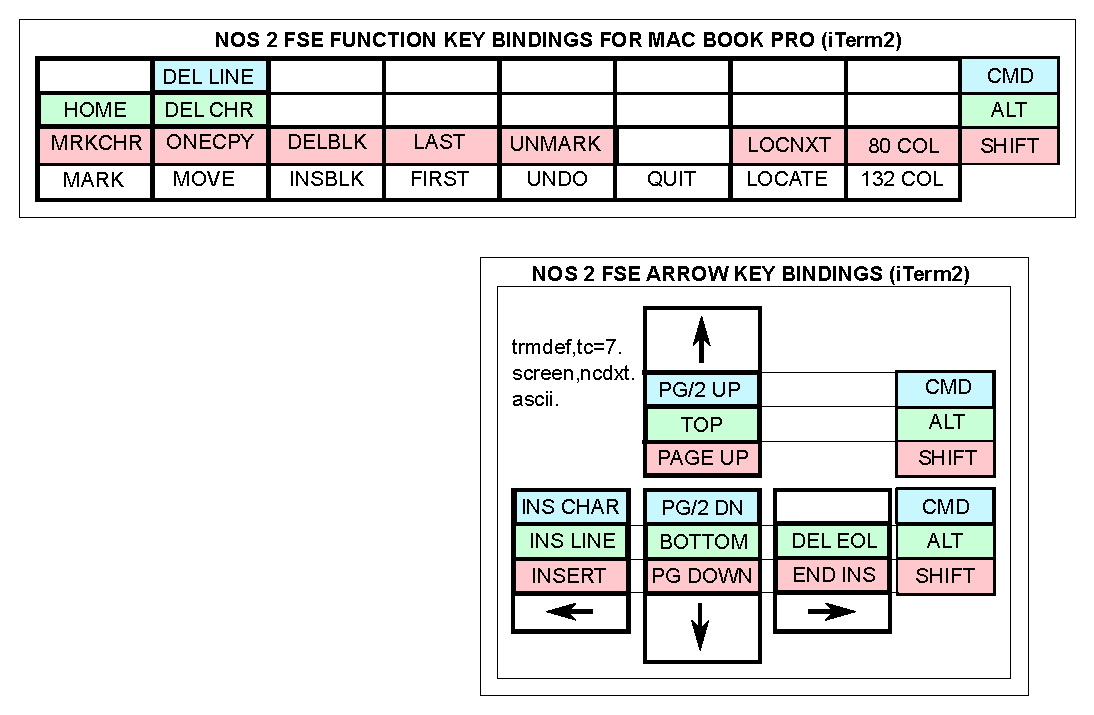
\includegraphics[scale=0.9]{../extras/iTerm2/fse-mac-iterm2.eps}
	\caption{Key definitions for iTerm2 on a laptop}
	\label{fig:it2map}
\end{figure}

\newpara
The key mappings this implements are shown in Figure~\ref{fig:it2map}. You do get used to them \ldots eventually!

\subsection{Alacritty for NOS 2.8}
Alacritty is an open source terminal emulator, perhaps best known for being written in Rust and for being very fast. Neither of these
`claims to fame' are particularly relevant, but it is a very good, cross-platform, terminal emulator. It is available here:\\
\url{https://github.com/alacritty/alacritty}.

\newpara
There are two Bash shell scripts in \texttt{extras/alacritty} that run Alacritty with suitable set-ups, one for desktop machines with full
size keyboards and one for laptops. 
\begin{itemize}
\item \texttt{nosterminal-desktop.sh} is for full size keyboards. The key mapping is the same as for Xterm, shown in Figure~\ref{fig:nost}.
\item \texttt{nosterminal-laptop.sh} is for laptop keyboards. The key mapping is the same as for iTerm2, shown in Figure~\ref{fig:it2map}.
\end{itemize}

\newpara
Although I've used iTerm2 on macOS and Xterm on Linux since I started using NOS, Alacritty may replace them both going forward.

\end{document}